\documentclass[twocolumn, a4paper, 10pt]{article}
\usepackage[utf8]{inputenc}
\usepackage[T1]{fontenc}
\usepackage{lmodern}
\usepackage{listings}
\usepackage{makeidx}
\usepackage[toc, page]{appendix}
\usepackage{float}
\usepackage{lscape}
\usepackage{csquotes}
\usepackage{soul}
\usepackage{textcomp}
\usepackage{gensymb}
\usepackage{pdfpages}
\usepackage{caption}
\usepackage{subcaption}
\usepackage{url}
\lstset{
	keywords={SELECT, WHERE, COLUMNS, ROWS, ON, MEMBER, WITH, FROM, ALL, CROSSJOIN, TOPCOUNT, ASC, DESC, AS, PARENT, CURRENTMEMBER, CHILDREN, PREVMEMBER, NEXTMEMBER, ORDER, RANK, GENERATE},
	keywordstyle=\color{red}\bfseries
}
% \usepackage{geometry}
\usepackage[left=20mm, right=20mm, top=25mm, bottom=25mm]{geometry}
\usepackage{rotating}
\usepackage[section]{placeins}
\usepackage{chngcntr,array}
\usepackage{graphicx}
\usepackage{lscape}
\usepackage{dirtree}
\usepackage[
	breaklinks=true,
	colorlinks=true,
	linkcolor=blue,
	urlcolor=blue,
	citecolor=blue,
	bookmarks=true,
	bookmarksopenlevel=2
]{hyperref}
\usepackage{xcolor}
\usepackage{algorithm}
\usepackage{algpseudocode}
\usepackage{amsmath}
\usepackage{amsfonts}
\usepackage{amssymb}

\title{
	Machine Learning
	\\-\\
	Supervised Learning
}
\author{
	\href{mailto:brandon.alves@gatech.edu}{Brandon Alves}
}
\date{\today}

\begin{document}
	\maketitle
	\tableofcontents
	% \listoffigures
	\section{Introduction}
		In this article, I will present the results of various Supervised Learning methods applied on two classification problems. Those methods are :
		\begin{itemize}
			\item Decision Trees with some form of pruning
			\item Neural Networks
			\item Boosting
			\item Support Vector Machines
			\item K-Nearest Neighbors
		\end{itemize}
		For each of them, I will discuss the results obtained, the pros and cons of using them, and the parameters that were used. I will also discuss the results when applying the methods on the two different datasets. At the end I will also compare the methods between them and highlight the best one for each dataset.

		I will present many plots on this report to show the evolution of the accuracy depending on some parameters. Those plots will be presented in the following way : the hard line represents the median precision value for a given parameter value while the tint area goes from the minimum to the maximum precision value for the given parameter value.
		% The error bar graph will follow the same convention with the center point representing the median value and the error bar going from minimum to maximum values.

		The experiments on this report were performed on a computer with the following specifications :
		\begin{itemize}
			\item CPU : Intel(R) Core(TM) i7-9750H CPU @ 2.60GHz, 6 cores, 12 threads
			\item RAM : 16GB DDR4
			\item GPU : NVIDIA Quadro P620
		\end{itemize}
	\section{Datasets}
		In this article, I will learn over two datasets :
		\begin{itemize}
			\item \href{https://www.kaggle.com/code/sngkadam/credit-card-fraud-detection/data}{Credit Card Fraud}
			\item \href{https://www.kaggle.com/c/the-insa-starcraft-2-player-prediction-challenge/data}{Starcraft II}
		\end{itemize}
		\subsection*{Credit Card Fraud}
			This dataset is a credit card fraud detection dataset. The dataset contains transactions made by credit cards in September 2013 by European cardholders. This dataset presents transactions that occurred in two days, where we have 492 frauds out of 284,807 transactions. The dataset is highly unbalanced, the positive class (frauds) account for 0.172\% of all transactions. It contains only numerical input variables which are the result of a PCA transformation. The only features which have not been transformed with PCA are \textit{Time} and \textit{Amount}. Feature \textit{Time} contains the seconds elapsed between each transaction and the first transaction in the dataset. The feature \textit{Amount} is the transaction amount. Feature \textit{Class} is the response variable and it takes value 1 in case of fraud and 0 otherwise.

			The training dataset contains between 10 000 and 210 000 transactions to evaluate how the training size can impact the results of the leaning process. The test dataset contains 236 transactions from the remaining samples that are not in the testing set. Half of the test dataset is composed of frauds and half of it is composed of non-fraud transactions. I have chosen that ratio in order to compare the ressults of the two datasets.
		\subsection*{Starcraft II}
			This dataset is composed of recorded competition games from the Starcraft II game. For each games, the dataset provides the player name and the player actions at a given time for a set of 30 different actions. The purpose is to find the player names having only the actions recorded.

			To allow all the medels to use that dataset, a number of feature is precomputed on it, such as the first time of each action or the average action per minute rate. This sum up into 72 different features for 200 class splits on 1950 games on the training set and 884 on the testing one. The training and testing set are constructed so that the same proportion are applied to each class to ensure that every class are represented on both datasets. The train dataset is then randomly flushed to allow to crop it for training and still have the possibility to have every class.

			The difficulty of this dataset is in hight number of different classes and the few numbers of example. There is 24 classes of the data set that have only 1 example to train from with an average of less than 10 per class. In addition, the dataset is noisy, some players appear under more than one pseudo and so some classes are very similar.

		\subsection*{Scaling}
			Some methods require the data to be scaled between 0 and 1. Both the training and the testing datasets are scaled between 0 and 1. The scaling is done by dividing each value by the maximum value of the dataset. The scaling is done on the training dataset and then applied on the testing dataset.
	\section{Decision Trees with some form of pruning}
		In that section I will present the results obtained when using Decision Trees with some form of pruning. We will here discuss the influence of different parameters :
		\begin{itemize}
			\item The maximum depth of the tree;
			\item The minimum number of samples required to split an internal node;
			\item The size of the training set.
		\end{itemize}

		We begin by finding the limit of our classifier. That limit can be of two natures : overfiting or a flat level on both training and test accuracy. Figure \ref{tree:train_vs_test} represents those limits.

		On figure \ref{tree:cc_train_vs_test}, we can see that the Decision Tree method quickly overfits. Indeed the training accuracy quickly rise above 99\% while the test accuracy decreases to reach around 0.87\%. We can notice that the best score is obtained for a maximum depth value of 1. Also the score considerably decreases for a maximum depth value of bigger than 3. therefore we can conclude that only 1 out of the 28 dimensions of the input space is relevant for the classification output.

		On figure \ref{tree:sc_train_vs_test}, we can notice that the classifier does not overfit. Although the training accuracy sometimes succeeds to reach 100\%, the test accuracy stays on a flat level around 0.75\%, meaning that increasing the maximum depth further does not impact the score of the classifier.

		\begin{figure}[]
			\centering
			\begin{subfigure}[]{0.8\columnwidth}
				\centering
				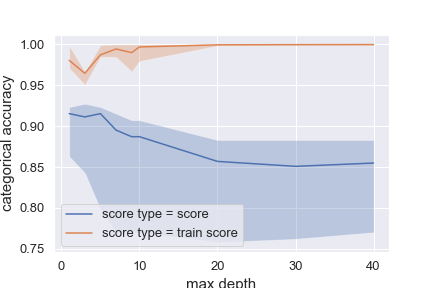
\includegraphics[width=\linewidth]{../graphics/tree_creditcard_max_depth_score_type_score_type.png}
				\caption{Accuracy for train and test credit-card datasets}
				\label{tree:cc_train_vs_test}
			\end{subfigure}
			\begin{subfigure}[]{0.8\columnwidth}
				\centering
				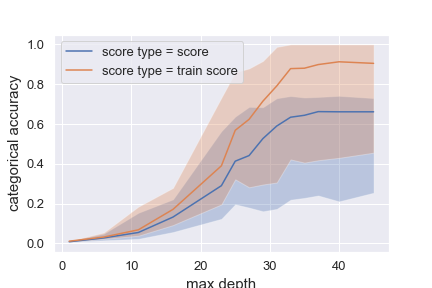
\includegraphics[width=\linewidth]{../graphics/tree_starcraft_max_depth_score_type_score_type.png}
				\caption{Accuracy for train and test Starcraft datasets}
				\label{tree:sc_train_vs_test}
			\end{subfigure}
			\caption{Evolution of the decision tree classifier accuracy according to the maximum depth of the tree}
			\label{tree:train_vs_test}
		\end{figure}

		Let's discuss now the influence of the size of the training set on the accuracy of the classifier. Figure \ref{tree:train_size_score_type_score_type} represents the accuracy of the classifier according to the size of the training set for the credit-card dataset. As expected the accuracy of the classifier decreases when the size of the training set decreases. The accuracy of the classifier is also impacted by the maximum depth of the tree. Indeed, the score for all the different sizes of the training set is almost the same when the maximum depth is around 1, whereas the score differs a lot when the maximum depth of the tree increases. We can also notice that the training set with 160 000 samples gives better results than the trainingset with 210 000 samples. This is probably due to the fact that the training set with 160 000 samples is more balanced than the training set with 210 000 samples, meaning that when adding those 50 000 samples, we probably introduce some noise in the training set.

		On the Starcraft sataset, we can see on figure \ref{tree:sc_train_size_score_type_score_type} that the accuracy of the classifier is also impacted by the size of the training set. Once again on that dataset there is no overfitting in the learning process. We can notice that the evolution of the gap between each step seems to evolve exponentially. But that comportment is mostly due to the classes not represented on the training set when dealing with few randomly chosen data for training. The standard deviation of accuracy is also reduced by the augmentation of the training set size. Indeed, the more data we consider, the less important fine-tuning the meta parameters is : the classifier will learn the best way to use that parameters and will so end up with similar results than another classifier with slightly different parameters.

		\begin{figure}[]
			\centering
			\begin{subfigure}[]{0.8\columnwidth}
				\centering
				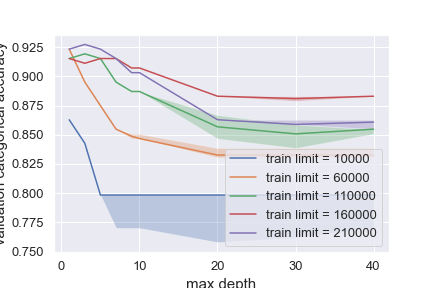
\includegraphics[width=\linewidth]{../graphics/tree_creditcard_max_depth_score_type_train_limit.png}
				\caption{Accuracy for train and test credit-card datasets}
				\label{tree:cc_train_size_score_type_score_type}
			\end{subfigure}
			\begin{subfigure}[]{0.8\columnwidth}
				\centering
				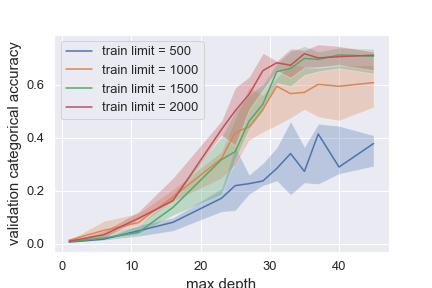
\includegraphics[width=\linewidth]{../graphics/tree_starcraft_max_depth_score_type_train_limit.png}
				\caption{Accuracy for train and test Starcraft datasets}
				\label{tree:sc_train_size_score_type_score_type}
			\end{subfigure}
			\caption{Evolution of the decision tree classifier accuracy according to the size of the training set}
			\label{tree:train_size_score_type_score_type}
		\end{figure}

		The last parameter I will discuss is the minimum number of samples required to split an internal node. That variation is displayed on figure \ref{tree:min_samples_split_score_type_score_type}. In the case of the credit-card dataset, we can see that the accuracy of the classifier is only impacted by the minimum number of samples required to split an internal node when overfiting. In Starcraft dataset, we see that this paramet has a little influence even if smaller than the over parameters.  In that particular case, this sort of pruning only led to decrease the accuracy of the classifier on the test set. This is probably caused by sometimes the very few data available per class, and at the same time do not prevent overfitting as the only overfitting possible here is due to the few data available.

		Decision Tree is the faster method compared with all the other ones. To get those results and generate the data associated with, it took 28 seconds. The full run coun 208 leanr and test cycles, which gives an average of 279 milliseconds per cycle. That is two time faster than KNN.

		The decision tree classifier performs pretty well as seen above. But that method does not perform very well on highly dimensional datasets. To resolve that problem, Random Forrest can be used. Random Forrest is a method that uses multiple decision trees to classify the data. The method is based on the idea that a large number of relatively uncorrelated classifiers (trees) operating as a committee will outperform any of the individual classifiers. The method is also known as bagging.

		\begin{figure}[]
			\centering
			\begin{subfigure}[]{0.8\columnwidth}
				\centering
				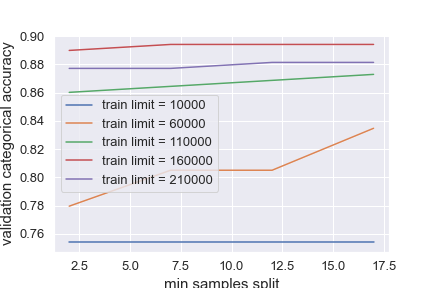
\includegraphics[width=\linewidth]{../graphics/tree_creditcard_min_samples_split_score_type_train_limit.png}
				\caption{Accuracy for train and test credit-card datasets}
				\label{tree:tree_creditcard_min_samples_split_score_type_train_limit}
			\end{subfigure}
			\begin{subfigure}[]{0.8\columnwidth}
				\centering
				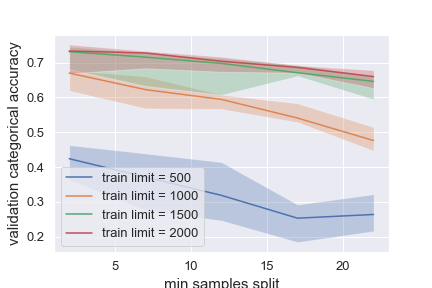
\includegraphics[width=\linewidth]{../graphics/tree_starcraft_min_samples_split_score_type_train_limit.png}
				\caption{Accuracy for train and test Starcraft datasets}
				\label{tree:tree_starcraft_min_samples_split_score_type_train_limit}
			\end{subfigure}
			\caption{Evolution of the decision tree classifier accuracy according to minimum number of samples required to split an internal node}
			\label{tree:min_samples_split_score_type_score_type}
		\end{figure}
	\section{Neural Networks}
	\section{Boosting}
	\section{Support Vector Machines}
	\section{K-Nearest Neighbors}
		Here I will discuss the results obtained using a K-Nearest Neighbors classifier. We will see the influence on the accuracy of the classifier of :
		\begin{itemize}
			\item The number of neighbors
			\item The distance metric (p-norm)
			\item The size of the training set
		\end{itemize}
		By design, the accuracy on the training set is always 100\% for KNN, so I will not display it on the plots.

		\begin{figure}
			\centering
			\begin{subfigure}[]{0.8\columnwidth}
				\centering
				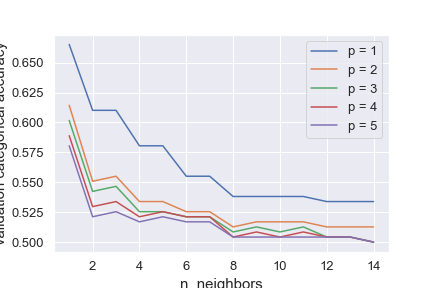
\includegraphics[width=\linewidth]{../graphics/knn_creditcard_neighbors.png}
				\caption{Evolution of accuracy according to the number of neighbors used for the classification on the credit-card fraud dataset, with $train\_limit=90000$}
				\label{knn:knn_cc_neighbors}
			\end{subfigure}
			\begin{subfigure}[]{0.8\columnwidth}
				\centering
				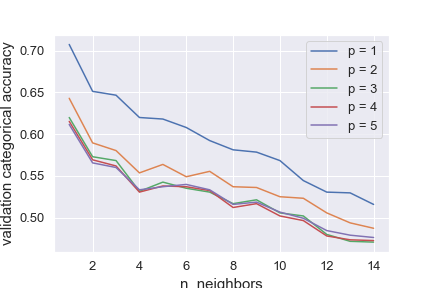
\includegraphics[width=\linewidth]{../graphics/knn_starcraft_neighbors.png}
				\caption{Evolution of accuracy according to the number of neighbors used for the classification on the Starcraft dataset, with $train\_limit=2000$}
				\label{knn:knn_sc_neighbors}
			\end{subfigure}
			\begin{subfigure}[]{0.8\columnwidth}
				\centering
				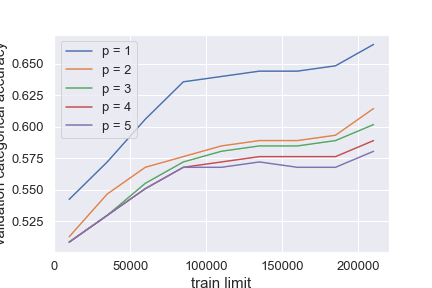
\includegraphics[width=\linewidth]{../graphics/knn_creditcard_train_limit.png}
				\caption{Evolution of accuracy according to the number of training examples on the credit-card fraud dataset, with $n\_neighbors=1$}
				\label{knn:knn_cc_train_limit}
			\end{subfigure}
			\begin{subfigure}[]{0.8\columnwidth}
				\centering
				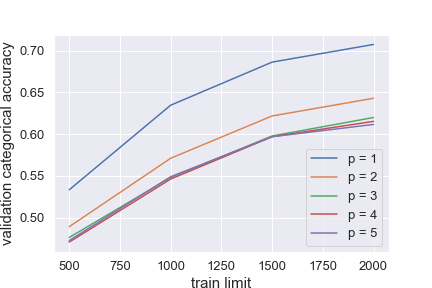
\includegraphics[width=\linewidth]{../graphics/knn_starcraft_train_limit.png}
				\caption{Evolution of accuracy according to the number of training examples on the Starcraft dataset, with $n\_neighbors=1$}
				\label{knn:knn_sc_train_limit}
			\end{subfigure}
			\caption{Evolution of the KNN classifier on the test set with different parameters}
			\label{knn:knn}
		\end{figure}

		On figure \ref{knn:knn}, I present the effect of those parameters on the classification score.
		First, we can notice that the norm used for the distance metric has a consequent influence on the classification accuracy. The accuracy is better when using the Manhattan norm ($p = 1$). This is not a surprise as higher norm are generally inadequate to measure distances on highly dimensional spaces.

		On figures \ref{knn:knn_cc_neighbors} and \ref{knn:knn_sc_neighbors}, we can see that the accuracy of the classifier is better for a small number of neighbors. This is not a surprise as both datasets have very few examples in each classes. KNN is a non-parametric classifier. It is not able to generalize the data, so it is better to use a small number of neighbors. We usually increase the research perimeter to be more resilient to noise but here the data do not allow us such a liberty. This is particularly true in the
		credit card dataset where the fraud are really close to legal transactions.

		On figures \ref{knn:knn_cc_train_limit} and \ref{knn:knn_sc_train_limit}, we can see that the accuracy of the classifier is better for an important number of training examples. Also the learning process don't overfit. However, on figure \ref{knn:knn_cc_train_limit}, for the credit-card datatset, we notice that there is a flat zone where the accuracy is pretty much constant. This is due to the fact that the number of frauds is very low compared to the number of legal transactions. I imagine that the samples added to the training set during that flat are mostly similar to previous ones. This is why the accuracy is not really increasing.

		Concerning time efficiency, the KNN classifier achieve a correct performance. On the Starcraft dataset, it takes 2m31s to run 280 times the learn and test process with the parameters explored above. KNN uses multiple thread to perform the classification task.

		In comparison with the other methods, KNN does not perform very well. Having a discussion with an expert of the dataset would be a godd idea for designing a distance metric that is better suited to the problem. Indeed, the distance metric is the key to the success of KNN. So it is important to choose the most appropriate one.
	\section{Conclusion}

\end{document}
